%% amssamp1.tex is nearly lidentical to amssamp2.tex, except
%% that amssamp2.tex uses the [twocol] option to produce
%% two-column text. Note that the figures and tables need to be
%% placed in text nearthe first callout, not at the end of the 
%% document. Also note that star form is used for figures
%% and tables.
\documentclass[twocol]{ametsoc}

%%%%%%%%%%%%%%%%%%%%%%%%%%%%%%%%
%%% To be entered only if twocol option is used
\journal{jtech}

%  Please choose a journal abbreviation to use above from the following list:
% 
%   jamc     (Journal of Applied Meteorology and Climatology)
%   jtech     (Journal of Atmospheric and Oceanic Technology)
%   jhm      (Journal of Hydrometeorology)
%   jpo     (Journal of Physical Oceanography)
%   jas      (Journal of Atmospheric Sciences)	
%   jcli      (Journal of Climate)
%   mwr      (Monthly Weather Review)
%   wcas      (Weather, Climate, and Society)
%   waf       (Weather and Forecasting)
%   bams (Bulletin of the American Meteorological Society)
%   ei    (Earth Interactions)

%%%%%%%%%%%%%%%%%%%%%%%%%%%%%%%%
%Citations should be of the form ``author year''  not ``author, year''
\bibpunct{(}{)}{;}{a}{}{,}

\title{Smoothing and Interpolating Noisy GPS Data with Tension Splines}

\authors{Jeffrey J. Early\correspondingauthor{Jeffrey J. Early, NorthWest Research Associates, 
				4118 148th Ave NE, Redmond, WA 98052.} and Adam Sykulski}

\affiliation{NorthWest Research Associates} 

\email{jearly@nwra.com}

\abstract{We develop a technique for smoothing and interpolating noisy GPS data using B-splines with tension. We show how the tension condition routinely employed in smoothing splines can be restated as a maximum likelihood problem and then how the tension parameter can be chosen based on physical reasoning. The GPS errors appear to be non-Gaussian, so we use a t-distribution in the maximum likelihood.  }

\usepackage{tensor}
\DeclareMathOperator{\Tr}{Tr}

\begin{document}

\maketitle

%%%%%%%%%%%%%%%%%%%%%%%%%%%%%%%%%%%%%%%%%%%%%%%%%%%%%%%%%%%%%%%%%%%%%
% MAIN BODY OF PAPER
%%%%%%%%%%%%%%%%%%%%%%%%%%%%%%%%%%%%%%%%%%%%%%%%%%%%%%%%%%%%%%%%%%%%%
\section{Introduction}
Global positioning system receivers (now commonly referred to as `a GPS') are used in literally billions of devices around the the world to track positions. The quality of the position data can be quite good, with accuracies down to a few meters, but real world effects (such as atmospheric conditions sky blockages) can significantly increase the errors \citep{faa2016-report}. Kalman filters are often employed to reduce these errors because they can be run in real time \citep{brown1997-book}. Here we consider an  approach using smoothing B-splines to control errors for data that has been collected and archived.

The data shown here was collected from from oceanic surface \emph{drifters}, floating buoys with drogues tethered 15-30 meters below the ocean surface, depending on the particular experiment. In the past, these drifters have used Argos positioning system which has significantly poorer temporal coverage and position accuracy \citep{elipot2016-jgr}, but recently more surface drifters have employed GPS receivers and transmitted their data back through Argos or Iridium satellites. The GPS receiver sits on the surface buoy and collects position data, but because of atmospheric conditions or ocean waves, the receivers are sometimes unable to obtain a position, or when they do, it is highly inaccurately. Thus, despite nominal accuracies of a few meters, it is often the case that some positions are off by more than 1000 meters.

In addition to correcting the position errors, it is also important to interpolate the data to a regular grid. Although the sampling period of a GPS receiver can be fixed, because of missing data and time to to acquire signals, the sampling can be quite irregular.  Many analysis techniques require regular sampling (e.g., a Fourier transform) and so it is necessary to interpolate the signal onto a regular grid. The approach taken here is not to simply discard poor data, but also to interpolate the position.

The primary dataset considered here will be nine surface drifters that were deployed in the Sargasso Sea in the summer of 2011. These particular drifters were part of the LatMix experiment \citep{shcherbina2015-bams} and recorded data at approximately 30 minute intervals over the course of a week before being retrieved.

The drifter positions are bivariate time series data given as either projected coordinates $(x_i, y_i)$ or longitude/latitude $(\phi_i, \theta_i$) at times $t_i$. The goal is to create a model of position $(x(t),y(t))$ that is continuous in $t$, and perhaps even continuous for a higher derivative---such as velocity or acceleration---that best matches the data given an assumed set of errors.

This manuscript is written to serve as a practical guide to smoothing noisy GPS data. As such, it begins by reviewing how to use B-splines \emph{interpolate} data to a continuous time series and then using maximum likelihood to \emph{smooth} the data in order to remove the noise in the positions. This is shown to be equivalent to using a tensioned smoothing spline. We demonstrate a new method for choosing an optimal smoothing parameter assuming Gaussian position errors. Finally, we show how the GPS errors are not Gaussian distributed, but t-distributed. We show how to implement our technique for this particular case.

%%%%%%%%%%%%%%%%%%%%%%
%
\section{Interpolation}
%
%%%%%%%%%%%%%%%%%%%%%%

\begin{figure*}[t]
  \centerline{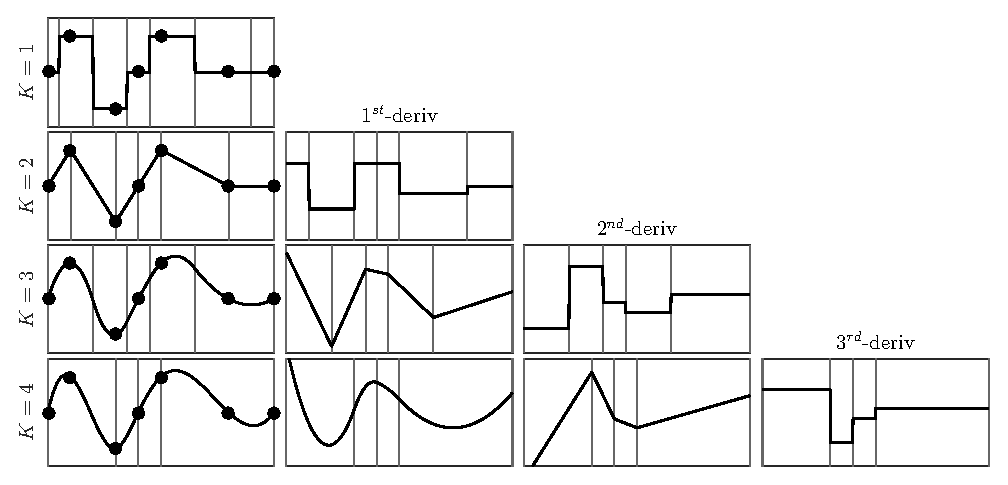
\includegraphics[width=39pc,angle=0]{interpolation}}
  
  \caption{This shows an example of interpolating between 7 data points. The data points are shown as circles, and the interpolated function is shown as a solid black lines. We show four different orders of interpolation $K=1..4$ (rows) and their nonzero derivatives (columns). The thin vertical grey lines are the knot points.}
  \label{interpolation}
\end{figure*}

Assume that we are given $N$ observations of a particle position $(t_i,x_i)$ with no errors. The simplest possible form of interpolation would be a nearest neighbor method that assigns the position of the particle to the nearest observations in time. The resulting interpolated function $x(t)$ is a polynomial of \emph{order} $K=1$ (piecewise constant), shown in the top row of figure \ref{interpolation}. The next level of sophistication is to assume a constant velocity between any two observations and use that to interpolate positions between observations, second row of figure \ref{interpolation}. This also means that we now have a piecewise constant function $\frac{dx}{dt}$ that represents the velocity of the particle, shown in the second row, second column of figure  \ref{interpolation}. This is a polynomial function of order $K=2$.

It is slightly less obvious how to proceed to a polynomial of order $K=3$. With $N$ data points we can construct a piecewise constant acceleration (the second derivative) using the $N-2$ independent accelerations, but where to place $\emph{knot points}$ that define the boundaries of the regions and how to maintain continuity is slightly less clear. The approach taken here is to use B-splines.

%%%%%%%%%%%%%%%%%%%%%%
\subsection{B-Splines}
%%%%%%%%%%%%%%%%%%%%%%

A B-spline (or basis spline) of \emph{order} $K$ (\emph{degree} $S=K-1$) is a piecewise polynomial that maintains nonzero continuity across $S$ knot points. The knot points are a nondecreasing collection of points in time that we will denote with $\tau_i$. The basic theory is well documented in \citet{deboor1978-book}, but here we will present a reduced version specifically tailored to our needs.

The $m$-th B-spline of order $K=1$ is defined as,
\begin{equation}
X^1_m(t) \equiv \begin{cases}
1      & \text{if $ \tau_m \leq t < \tau_{m+1}$}, \\
0     & \text{otherwise}.
\end{cases}
\end{equation}
This is the rectangle function as shown in the first row, first column of figure \ref{bsplines}. If we are given $P$ knot points, then we can construct $P-1$ B-splines of order $K=1$, although notice that if a knot point is repeated this will result in a splines that is zero everywhere. To represent an interpolating function $x(t)$ for the $N$ observations of a particle position $(t_i,x_i)$ we define $N+1$ knot points as,
\begin{equation}
\tau_m = \begin{cases}
t_1      & \text{$m=1$}, \\
t_{m-1} + \frac{t_{m-1}-t_m}{2}	  & \text{$1<m \leq N$}\\
t_N     & \text{$m>N$}.
\end{cases}
\end{equation}
This will create $N$ independent basis functions that provide support for the region $t_i \leq t \leq t_N$ (provided the last spline is defined to include the last knot point). The interpolating function $x(t)$ is defined as $x(t) \equiv  X^1_m(t) \xi^m$ where the coefficients $\xi^m$ are found by solving $X^1_m(t^i) \xi^m = x^i$. The result of this process is shown in figure \ref{interpolation} for 7 irregularly spaced data points.

All higher order B-splines are defined by recursion,
\begin{equation}
X^K_m(t) \equiv \frac{t - t_m}{t_{m+K-1} - t_m} X^{K-1}_m(t) + \frac{t_{m+K}-t}{t_{m+K} - t_{m+1}} X^{K-1}_{m+1}(t).
\end{equation}
This recursion formula takes two neighboring lower order splines and ramps the left one up over its nonzero domain and ramps the right one down over its nonzero domain. The result of this process is to create splines that span across one additional knot point at each order, and maintain continuity across one more derivatives. Examples are shown in figure \ref{bsplines}.

Any knot points that are repeated $T$ times will result in an a total of $T-1$ splines of order one that are everywhere zero. This has the effect of introducing discontinuities in the derivatives for higher order splines. For our purposes, we will only use this feature to prevent higher order splines from crossing the boundaries. For $K=2$ order splines we will use $N+2$ knot points at locations,
\begin{equation}
\tau_m = \begin{cases}
t_1      	& \text{$m \leq 2$}, \\
t_{m-1}	& \text{$2 < m < N$}\\
t_N 		& \text{$m \geq N$}.
\end{cases}
\end{equation}
This creates a knot point at every observation point, but repeats the first and last knot point. This has the effect of terminating the first and last spline at the boundary and creating $N$ second order B-splines, $X^2_m(t)$. Once again the interpolating function $x(t)$ is defined as $x(t) \equiv  X^2_m(t) \xi^m$ where the coefficients $\xi^m$ are found by solving $X^2_m(t^i) \xi^m = x^i$. The second row of figure \ref{interpolation} shows an example.

This process can be continued to higher and higher order B-splines. For splines that are of \emph{even} order, we create $N+K$ knots points with
\begin{equation}
\tau_m^{\text{$K$-even}} = \begin{cases}
t_1      	& \text{$m \leq K$}, \\
t_{m-K/2}	& \text{$K < m < N$}\\
t_N 		& \text{$m \geq N$}
\end{cases}
\label{even-knots}
\end{equation}
and for splines that are \emph{odd} order, we create $N+K$ knot points with,
\begin{equation}
\tau_m^{\text{$K$-odd}} = \begin{cases}
t_1      	& \text{$m \leq K$}, \\
t_{m-\frac{K+1}{2}} + \frac{t_{m-\frac{K+1}{2}}-t_{m-\frac{K+1}{2}+1}}{2}	& \text{$K < m \leq N$}\\
t_N 		& \text{$m > N$}
\end{cases}
\label{odd-knots}
\end{equation}
The knot points are chosen specifically to create $N$ splines for the $N$ data points such that the interpolated function $x(t)$ crosses all $N$ observations $(t_i,x_i)$. Examples are shown in figure \ref{interpolation}.

\begin{figure}
  \centerline{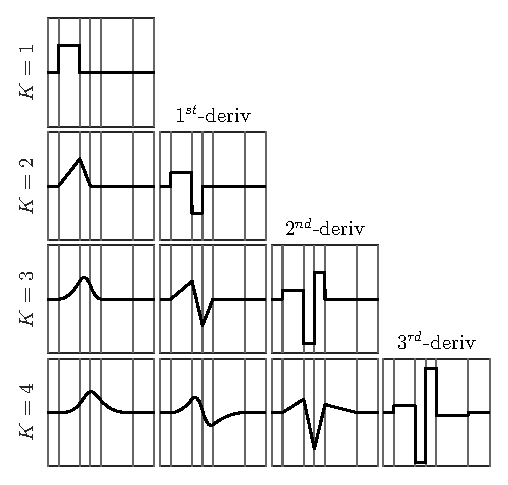
\includegraphics[width=19pc,angle=0]{bsplines}}
  \caption{This shows an example B-spline and its derivatives (columns) for orders $K=1..4$ (rows).}
  \label{bsplines}
\end{figure}


%%%%%%%%%%%%%%%%%%%%%%
%
\section{Maximum Likelihood}
%
%%%%%%%%%%%%%%%%%%%%%%

Using B-splines we now have a mechanism for generating continuous paths given a set of observations, but each observation, $x_i$, differs from the true value, $x(t_i)$, by some noise, $\epsilon_i \equiv x_i - x(t_i)$. The goal now is to find a path $x(t)$ that is not contaminated by the noise.

The approach taken here is to use maximum likelihood. The central idea of maximum likelihood is to ask ``Given a particular path $(x(t),y(t))$, what is the probability that this dataset $(t_i,x_i, y_i)$ could have occurred?'' \citep{press1992-book}. The goal is then to find the path that is most likely to have produced that dataset.

Conceptually we have two major pieces that we need to solve this problem:
\begin{enumerate}
\item we need to specify at least one probability distribution function (PDF) for some aspect of the signal or errors, and
\item we need to specify the form of the path (model).
\end{enumerate}

%%%%%%%%%%%%%%%%%%%%%%
\subsection{Error PDF}
%%%%%%%%%%%%%%%%%%%%%%

A typical starting point is to establish the probability distribution function (PDF) of the errors, $\epsilon_i$. The canonical example in one-dimension is to assume that the error in our position measurements are Gaussian and are therefore drawn from the following probability distribution
\begin{equation}
\label{gaussian_pdf}
p_g(\epsilon|\sigma_g) = \frac{e^{-\frac{1}{2}\frac{\epsilon^2}{\sigma_g^2}} }{\sigma_g \sqrt{ 2 \pi}}.
\end{equation}
This assumption alone places no assumptions on the signal itself, only on the structure of the noise.

The probability of the observed data given some model $x(t)$ is,
\begin{equation}
\label{max-gaussian}
P \sim \prod_{i=1}^{N}  \exp \left[ -\frac{1}{2} \left( \frac{x_i - x(t_i)}{\sigma_i} \right)^2 \right] \Delta x
\end{equation}
where $x_i$ represents the observations at time $t_i$ with estimated error of $\sigma_i$.

Maximizing the probability function in equation \ref{max-gaussian} is also the same as minimizing its argument (called the penalty function),
\begin{equation}
\label{least-squares}
\phi = \sum_{i=1}^{N} \left( \frac{x_i - x(t_i)}{\sigma_i} \right)^2 .
\end{equation}
Stated in this way is plain to see that this is the same as asking for the `least-squares' fit of the errors.

%%%%%%%%%%%%%%%%%%%%%%
\subsection{Model}
%%%%%%%%%%%%%%%%%%%%%%

The model used here will be an interpolating B-spline representation of the data at some order $K$ with knot points generated by equations \ref{even-knots} and \ref{odd-knots}. Of course, we've chosen our knot points such that the model intersects each observations and this certainly maximizes equation \ref{max-gaussian} (and minimize equation \ref{least-squares}) because all the errors are zero, but the resulting distribution of errors (a delta function at zero) doesn't look anything like the assumed Gaussian distribution. Thus, if we want the error distribution that we get out to look like that which we assumed, it also necessary to \emph{constrain} the problem in some way. There are conceptually (at least) two ways of doing this, either 
\begin{enumerate}
\item specify a model with fewer degrees of freedom than data points, or
\item specify additional \emph{global} constraints on the model in the penalty function.
\end{enumerate}
These two may be equivalent. For example, you may decide the model is a straight line (with two degrees of freedom), or you could set a constraint that that the integral of the second derivative vanish.

We could easily create a model with fewer degrees of freedom than data points by simply removing and rearranging  some of the knot points generated by equations \ref{even-knots} and \ref{odd-knots}. This is certainly worth doing if the data is \emph{oversampled}, where expected distance traversed ($u_{\textrm{rms}}\Delta t$) between observation times ($\Delta t$) is less than the expected error $\sigma_x$. For the cases considered here, we are in an \emph{under-sampled} regime where the drifters have traveled far beyond their the expected error in the time between observations.

The other alternative, and the approach taken here, is to specify a global constraint on the model in the penalty function. In particular, we will use what is known as a smoothing spline.

%%%%%%%%%%%%%%%%%%%%%%
%
\section{Smoothing Spline}
%
%%%%%%%%%%%%%%%%%%%%%%

The smoothing spline augments the penalty function of equation \ref{least-squares} by adding a global constraint on the $m$-th derivative of the resulting function
\begin{equation}
\label{smoothing-spline}
\phi =  \sum_{i=1}^{N} \left( \frac{x_i - x(t_i)}{\sigma_i} \right) ^2 + \lambda_m \int_{t_1}^{t_N} \left(\frac{d^m x}{dt^m}\right)^2 \, dt.
\end{equation}
If $\lambda_m \rightarrow 0$ then this reduces to the least-squares fit in equation \ref{least-squares}, but if $\lambda_m \rightarrow \infty$ then this forces the model to an $m$-th order polynomial (e.g., when $m=2$, the model will forced to be a straight line because it has no second derivative). The smoothing spline was first introduced in modern form by \citet{reinsch1967-nm}, but according to \citet{deboor1978-book} the idea dates back to \citet{whittaker1923-pems}.

The one free parameter in this model, $\lambda_m$, is a relative weighting between the two terms in equation \ref{smoothing-spline} and choosing its optimal value will be deferred to section \ref{optimal_parameter}. For now, we show how these two terms are expected to scale statistically and physically.

%%%%%%%%%%%%%%%%%%%%%%
\subsection{Sample variance term}
%%%%%%%%%%%%%%%%%%%%%%

The first term of equation \ref{smoothing-spline} is proportional to the sample variance,
\begin{equation}
\hat{\sigma}^2  \equiv \frac{1}{N} \sum_{i=1}^{N} \left( x_i - x(t_i) \right) ^2,
\end{equation}
which is expected to scale like
\begin{equation}
\label{sample_variance}
\hat{\sigma}^2 = \frac{d-1}{d} \sigma^2
\end{equation}
where $d$ is the number of degrees of freedom (reference Adam? It's on the wikipedia page on Cochran's theorem). For a large number of degrees of freedom, $d$, the sample variance matches the true variance, but as will be discussed in section \ref{optimal_parameter}, this is generally not the case. This means that the first term in equation \ref{smoothing-spline} scales like $N \frac{d-1}{d}$.

This should be compared with our estimate for the sample mean, the error for which is expected to scale like $SE = \frac{\sigma}{\sqrt{d}}$.

%%%%%%%%%%%%%%%%%%%%%%
\subsection{Tension term}
%%%%%%%%%%%%%%%%%%%%%%

There is a very simple \emph{physical} interpretation for the second term in equation \ref{smoothing-spline}. Consider the case where $m=1$ so that the smoothing spline is a constraint on velocity. When averaged over the integration time, the integral produces the root mean square velocity, $u_{\textrm{rms}}$, which means that the second term scales like $u_{\textrm{rms}}^2 T$ where $T\equiv t_N-t_1$. This means that the penalty function becomes
\begin{equation}
\label{smoothing-spline-velocity}
\phi =  \sum_{i=1}^{N} \left( \frac{x_i - x(t_i)}{\sigma_i} \right) ^2 + \frac{d-1}{d} \frac{N}{u_{\textrm{rms}}^2 T} \int_{t_1}^{t_N} u^2(t) \, dt
\end{equation}
when the two terms are equally weighted by their expected values and thus $\lambda_1 = \frac{d-1}{d} \frac{N}{u_{\textrm{rms}}^2 T}$ or
\begin{equation}
\label{lambda}
\lambda_m = \frac{d-1}{d} \frac{N}{ \left(x^{(m)}_{\textrm{rms}}\right)^2 T}
\end{equation}
in general, where $x^{(m)}_{\textrm{rms}}$ is the root-mean-square of the $m$-th derivative.

The smoothing spline can be restated in terms of maximum likelihood. Assume that in addition to knowing about how the measurement errors are distributed, that we also know how the velocity of underlying physical process is distributed. For example, in geophysical turbulence it has been shown that the velocity probability distribution function is like a two-sided exponential (cite Bracco et al., 2000). Here we will consider the case where the velocity PDF is Gaussian. Stated as maximum likelihood, this means that at \emph{any given instant} (not just the times of observation) we expected the model velocity to look Gaussian. We can discretize the problem by sampling the velocity $Q$ at times $t_q = t_1 + q \Delta t_q$ where $\Delta t_q=\frac{t_N-t_1}{Q-1}$ and $q=0..Q-1$. The maximum likelihood is thus stated as,
\begin{equation}
\label{gaussian-max-likelihood}
\begin{split}
P \sim \prod^N _{i=1}\exp \left[ -\frac{1}{2} \left( \frac{x_i - x(t_i)}{\sigma_i} \right)^2 \right] \\\cdot \prod^{Q}_{q=1} \exp \left[  - \frac{1}{2} \left(  \frac{u(t_q)}{\sigma_u} \right)^2 \right] \Delta x.
\end{split}
\end{equation}
Writing this as a penalty function (after converting the product of exponentials into exponentials of sums), we have that
\begin{equation}
\phi =  \frac{d}{d-1} \frac{1}{N} \sum^N _{i=1}\left( \frac{x_i - x(t_i)}{\sigma_i} \right)^2 + \frac{1}{Q} \sum^{Q}_{q=1}  \left(  \frac{u(t_q)}{\sigma_u} \right)^2
\end{equation}
where we've renormalized the error PDF and the velocity PDF to have equal weighting regardless of number of points. Some simple rearranging gives you that,
\begin{equation}
\label{smoothing-spline-pdf}
\phi =\frac{d}{d-1}  \frac{1}{N} \sum^N _{i=1}  \left( \frac{x_i - x(t_i)}{\sigma_i} \right)^2 + \frac{1}{\sigma_u^2 T} \sum^{Q}_{q=1}  u^2(t_q) \Delta t_q.
\end{equation}
Apart from the discretization of the integral, equation \ref{smoothing-spline-velocity} is the same as \ref{smoothing-spline-pdf}. (need to fix the indices for Q).

The implication of this result is that adding tension to the penalty function is equivalent to assuming that one of the higher order derivatives in the model (e.g., velocity) is Gaussian. This is therefore making an assumption about the underlying \emph{physical process} of the model. This is in contrast to the first term which is entirely a statement about measurement noise.

%%%%%%%%%%%%%%%%%%%%%%
%
\section{Numerical Implementation}
%
%%%%%%%%%%%%%%%%%%%%%%

\begin{figure*}[t]
  \centerline{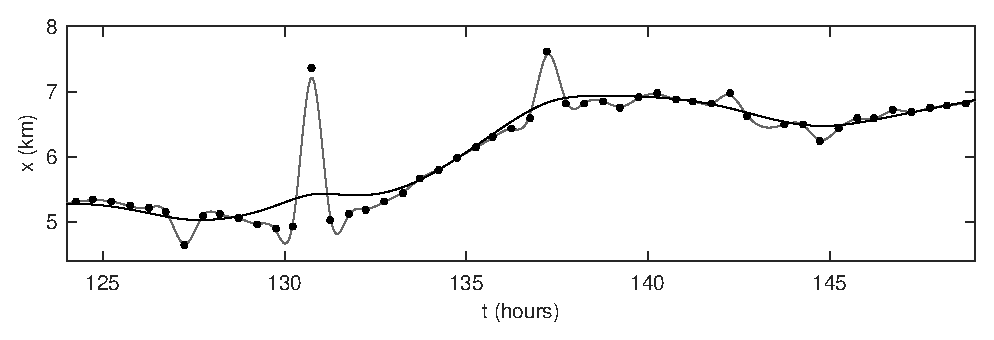
\includegraphics[width=39pc,angle=0]{gaussianfit}}
  
  \caption{An example of model fits assuming Gaussian errors with $\sigma=10$ meters. The black line shows a fit with high tension ($a_{\textrm{rms}}=2 \cdot 10^{-5}$ m$^2$/s), while the gray line shows a fit with  low tension ($a_{\textrm{rms}}=2 \cdot 10^{-4}$ m$^2$/s).}
  \label{gaussianfit}
\end{figure*}


The B-splines are generated using the algorithm described in \citet{deboor1978-book} with knot points determined by equations \ref{even-knots} and \ref{odd-knots}. The matrix $\mathbf{X}$ with components $X\indices{^i_m}$ denotes the $m$-th B-spline at time $t_i$. The first, second and third derivatives of the B-splines are denotes by $V\indices{^i_m}$, $A\indices{^i_m}$, $J\indices{^i_m}$, denoting velocity, acceleration, and jerk, respectively. In this notation the column vector $\xi^m$ represents the coefficients of the splines such that positions at time $t_i$ are given by $\hat{x}^i$ where $\hat{x}^i =  X\indices{^i_m} \xi^m$.

The discretized the penalty function is
\begin{equation}
\begin{split}
\phi = \left[ x^k - X\indices{^k_j} \xi^j \right]^{\textrm{T}} \left(\Sigma^{-1}\right)\indices{^k_i} \left[ x^i - X\indices{^i_l} \xi^l \right] \\
+ \lambda_1 \left[V\indices{^q_j} \xi^j \right]^{\textrm{T}} \left[ V\indices{^q_l} \xi^l \right]
\end{split}
\end{equation}
or
\begin{equation}
\phi = \left[ \mathbf{x} - \mathbf{X} \mathbf{\xi} \right]^{\textrm{T}} \Sigma^{-1} \left[ \mathbf{x} - \mathbf{X} \mathbf{\xi}\right]
+ \lambda_1 \left[\mathbf{V}\mathbf{\xi} \right]^{\textrm{T}} \left[ \mathbf{V}\mathbf{\xi} \right]
\end{equation}
where $\Sigma$ denotes the covariance matrix describing the measurement errors.

To find the coefficients that minimize this function, we take the derivative with respect to $\xi^m$, set it equal to zero, and solve for $\xi^m$,
\begin{equation}
\begin{split}
\xi^m = \left[ X\indices{_k_j} \left(\Sigma^{-1}\right)\indices{^k_i}  X\indices{^i_m} + \lambda_1 {A}\indices{^q_j}{A}\indices{^q_m} \right]^{-1} \\
\cdot x_k \left(\Sigma^{-1}\right)\indices{^k_i}   X\indices{^i_j}.
\end{split}
\label{solution}
\end{equation}
or
\begin{equation}
\mathbf{\xi} = \left[ \mathbf{X}^{\textrm{T}} \Sigma^{-1} \mathbf{X} + \lambda_1 \mathbf{V}^{\textrm{T}} \mathbf{V} \right]^{-1} \mathbf{X}^{\textrm{T}} \Sigma^{-1} \mathbf{x}
\end{equation}
This means that,
\begin{equation}
\mathbf{\hat{x}} = \mathbf{S_\lambda} \mathbf{x}
\end{equation}
where we've defined the smoothing matrix
\begin{equation}
\label{smoothing-operator}
\mathbf{S_\lambda} \equiv \mathbf{X} \left[ \mathbf{X}^{\textrm{T}} \Sigma^{-1} \mathbf{X} + \lambda_1 \mathbf{V}^{\textrm{T}} \mathbf{V} \right]^{-1} \mathbf{X}^{\textrm{T}} \Sigma^{-1}.
\end{equation}
which takes observations $\mathbf{x}$ to their smoothed values $\mathbf{\hat{x}}$.

The first matrix on the right hand side of equation \ref{solution} is $N\times N$ and fully invertible because the knots point were chosen such that each spline has at least one data point in its nonzero region. This is a nice feature because it means the solution will be well-behaved even if there is no tension.


%%%%%%%%%%%%%%%%%%%%%%
%
\section{Optimal parameters} \label{optimal_parameter}
%
%%%%%%%%%%%%%%%%%%%%%%

In the 50 years since \citet{reinsch1967-nm} was published, a number of different methods have been proposed for choosing the optimal value of $\lambda_m$. One approach is cross-validation \citep{wahba1978-jrss-b,craven1979-nm} which is essentially a form of bootstrapping, where the optimal parameter is determined by minimizing the error with data points not included in the fit. Another approach is to determine the number of degrees of freedom expected in the sample variance of equation \ref{sample_variance}. Both \citet{reinsch1967-nm} and \citet{teanby2007-mg} argue that the tension should be adjusted so that the sample variance is roughly the expected variance, $\hat{\sigma}^2 \sim \sigma^2$, but this assumes a large number of degrees of freedom. According to \citet{wahba1990-siam} this appears to overestimate the number of degrees of freedom. Different techniques for determining the degrees of freedom have been proposed, see for example \citet{cantoni2002-biom}.

We argue that the degrees of freedom, and therefore the tension, should vary based on the relative size of the measurement errors to the speed of motion. For example, if the position errors are only $1$ meter, but particle typically travels $10$ meters between measurements, then it is hardly justifiable to increase the tension so that the smoothing spline misses the observation points by $1$ meter. There is not enough statistical evidence to suggest that the true particle didn't go right through the observation point. On the other hand, if the position errors are  $1$ meter, but particle typically travels $10$ centimeters between measurements, nearby measurements are providing more information about the particle's true position during that time, so our estimate of the particles true position is closer to a mean of the nearby observations.

This idea can be made more rigorous by noting that one would consider change in position, $\Delta x$, statistically significant if exceeds the position errors, $\sigma_x$ by 2-3 factors. Assuming the physical process has a characteristic velocity scale, $u_{\textrm{rms}}$, we use this concept to define $\Gamma$ as
\begin{equation}
\Gamma_x \equiv \frac{3 \sigma_x}{u_{\textrm{rms}}\Delta t}
\end{equation}
where $\sigma_x$ is the standard deviation of positioning noise and $\Delta t$ is the typical time between observations. In terms of degrees of freedom, this argument suggests that $d = 1 + \Gamma$.

The quantity $\Gamma$ can also be interpreted as an interpolation condition. If $\Gamma<1$ then we are in the interpolation regime where the particle moves farther than the measurement noise between observations, and if $\Gamma >1$ we are in the smoothing regime where each observation is providing similar information to nearby observations.

Having established a value for $d$, we can computed $\lambda_m$ of equation \ref{lambda} directly. To do this we need an estimate of $u_{\textrm{rms}}$, in order to compute $\Gamma$, and $x^{(m)}_{\textrm{rms}}$ to properly normalize the tension. These quantities can be estimated from the various spectra of the observed signal, as will be shown below.

While that provides a good initial guess, we find that the more robust approach is to fix the degrees of freedom in the standard error estimate of the mean. In particular the variance of the mean for a Gaussian decreases with increasing degrees of freedom as $\sigma^2/d$. This quantity is, in fact, $\mathbf{S_\lambda} \Sigma$ for each observation. On average then, the number of degrees of freedom is,
\begin{equation}
d = \frac{N}{\Tr \left(\mathbf{S_\lambda} \Sigma \right) }.
\end{equation}
Adjusting the tension parameter such that,
\begin{equation}
1 + \frac{3 \sigma_x}{u_{\textrm{rms}}\Delta t} = \frac{N}{\Tr \left(\mathbf{S_\lambda} \Sigma \right) }.
\end{equation}
should provide nearly optimal tension.

%%%%%%%%%%%%%%%%%%%%%%
%
\section{Example Data}
%
%%%%%%%%%%%%%%%%%%%%%%

To test these ideas we generate synthetic velocity data from a Gaussian process known as the Matern, and then contaminate the positions with Gaussian noise.

Show plot of signal and error spectra.

Show a plot of optimal DOF value vs estimated DOF.

This process is chosen because it has physically desirable characteristics including a roll off at high frequencies and finite values at low frequencies. We choose values so that $\Gamma$ varies from approximately


%%%%%%%%%%%%%%%%%%%%%%
\section{Gaussian errors}
%%%%%%%%%%%%%%%%%%%%%%

Figure \ref{gaussianfit} shows the results of fitting to the observations assuming the errors are Gaussian. The error $\sigma$ is taken to be $10$ meters, as found in the analysis of GPS errors. Of course, there is really only one adjustable parameter so this choice is  irrelevant as we choose to fix $\sigma$ and adjust $a_{\textrm{rms}}$.  A reasonable estimate for a physically realistic acceleration can be found by noting that the largest signal is inertial, so if we take with $u \approx 0.1$ m/s this implies  that $a \approx u f_0$, or $a \approx 8 \cdot 10^{-6}$ m$^2$/s. Figure \ref{gaussianfit} shows two fits, one with relatively low tension (high $a_{\textrm{rms}}=2 \cdot 10^{-5}$ m$^2$/s) and one with relatively high tension (low $a_{\textrm{rms}}=2 \cdot 10^{-6}$ m$^2$/s).
\begin{figure*}[t]
  \centerline{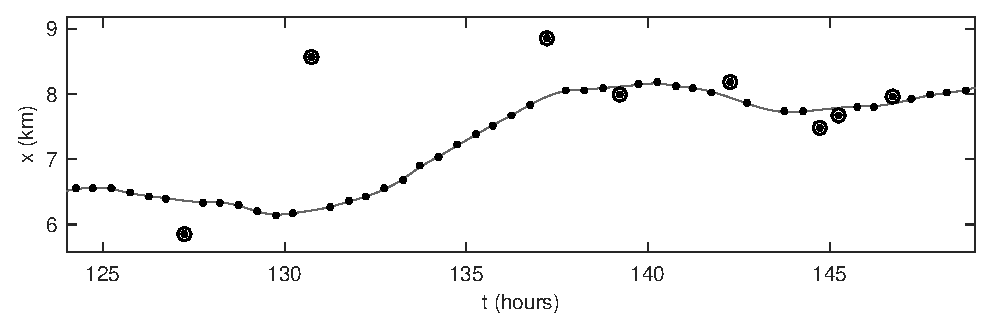
\includegraphics[width=39pc,angle=0]{tdistributionfit}}
  
  \caption{An example of model fits assuming errors following a t-distribution.}
  \label{tdistributionfit}
\end{figure*}

Increasing tension (by decreasing $a_{\textrm{rms}}$) reduces the variance in the resulting acceleration PDF because the model fits with large accelerations are considered unlikely. The has the effect of `pulling' the model fit further away from the observation points that would have otherwise resulted in larger accelerations. This also means that if the tension is increased too much, several successive points will be missed and there will now be correlation in errors. This is evident in figure \ref{gaussianfit} where the black line (high tension) fit stays to one side of the data for several successive points. On the other hand, decreasing the tension will improves the error correlation metric. The gray line (low tension) fit in figure \ref{gaussianfit} shows far more zero crossings. However, the low tension case also results in physical outliers---regions where the model fit makes large excursion that are clearly unphysical.

This autocorrelation sequence for the errors are shown in figure \ref{gaussianacf}. The high tension (black line) case shows a strong \emph{negative} correlation in the errors at lag 1, the opposite of what would be expected simply by looking at the correlation in the sign of the errors. This is because the autocorrelation sequence is weighted by variance and is therefore dominated by the effect of the outliers which do show a negative correlation with neighboring points. The low tension cause follows the same logic for lag 1, but shows a positive correlation at lag 2 where the spline `overshoots' the observed data.

The problem with using a Gaussian PDF for the errors is that there are no outliers. Values more than 4 or 5 $\sigma$ from the mean are effectively impossible. The solution is then to use some other distribution which will treat data points beyond a certain distance as outliers.

%%%%%%%%%%%%%%%%%%%%%%
%
\subsection{GPS Error PDF}
%
%%%%%%%%%%%%%%%%%%%%%%

We characterize the the GPS errors by considering data from a motionless GPS receiver allowed to run for 12 hours. The specific GPS receiver used for this test was not the same as the one used for the drifters but should produce errors similar enough for this analysis. The errors documented in the FAA GPS accuracy report (cite) are less comparable because they use superior antennas.

The position recorded by the motionless GPS are assumed to have isotropic errors with mean zero, which means that the positions themselves are the errors. The probability distribution function (PDF) of the combined $x$ and $y$ position errors are shown in figure \ref{motionless_error}.

The error distribution is first fit to a Gaussian probability distribution function (PDF),
\begin{equation}
\label{gaussian_pdf}
p_g(\epsilon|\sigma_g) = \frac{e^{-\frac{1}{2}\frac{\epsilon^2}{\sigma_g^2}} }{\sigma_g \sqrt{ 2 \pi}}.
\end{equation}
The best fit is produced by compute the standard deviation of the sample (Adam, citation?), which is found to be $\sigma_g \approx 10$ meters and shown as the gray line in figure \ref{motionless_error}. However, it is clear the error distribution shows much longer tails than the Gaussian PDF.

The Student t-distribution is a generalization of the Gaussian that produces longer tails where 
\begin{equation}
\label{student_pdf}
p_t\left(\epsilon |\nu,\sigma_t^2\right) = \frac{\Gamma\left( \frac{\nu + 1}{2} \right)}{\sigma_t \sqrt{\nu \pi} \Gamma\left(\frac{\nu}{2}\right)} \left( 1 + \frac{\epsilon^2}{\sigma_t^2 \nu} \right)^{-\frac{\nu+1}{2}}
\end{equation}
where the $\sigma_t$ parameter scales the distribution width and the $\nu$ parameter sets the number of degrees of freedom. The variance is $\textrm{var}(X)=\sigma_t^2 \frac{\nu}{\nu-2}$ and only exists for $\nu > 2$. The t-distribution is equivalent to the Gaussian distribution when $\nu \rightarrow \infty$. We find the best fit t-distribution to the data by maximizing the Kolmogorov-Smirnoff test. The best fit with parameters $\sigma_t \approx 8$ meters and $\nu \approx 5.5$ is shown as the black line in figure \ref{motionless_error}.

\begin{figure}
  \centerline{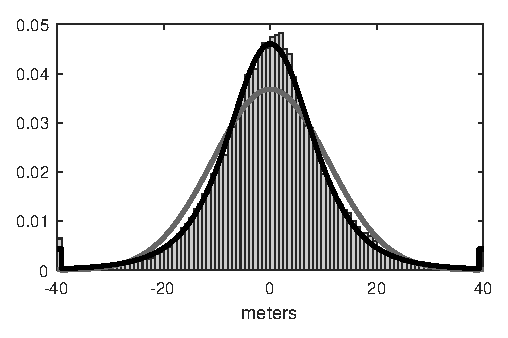
\includegraphics[width=19pc,angle=0]{motionless_error}}
  \centerline{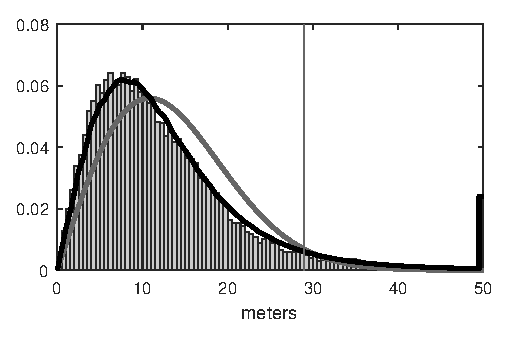
\includegraphics[width=19pc,angle=0]{motionless_distance_error}} 
  \caption{The top panel shows the position error distribution of the motionless GPS. The black line is the best fit t-distribution and the gray line is the best fit Gaussian distribution. The bottom panel shows the distance error distribution with the corresponding expected distributions from the Gaussian and t-distribution. The vertical line in the bottom panel shows the 95\% error of the t-distribution at about 29 meters.}
  \label{motionless_error}
\end{figure}

The \emph{position} error distributions also imply a combined \emph{distance} error distribution by computing $\epsilon_d = \sqrt{\epsilon_x^2 + \epsilon_y^2}$ and is shown in the lower panel of figure  \label{motionless_error}. For two independent Gaussian distributions this results in a Rayleigh distribution,
\begin{equation}
\label{rayleigh_pdf}
p_r(\epsilon_d|\sigma_g) = \frac{\epsilon_d}{\sigma_g^2 } e^{-\frac{1}{2}\frac{\epsilon_d^2}{\sigma_g^2}}.
\end{equation}
The distance distribution for two t-distributions is computed numerically.

%%%%%%%%%%%%%%%%%%%%%%
\section{Non-Gaussian errors}
%%%%%%%%%%%%%%%%%%%%%%

In practice it is challenging to use the Student t-distribution directly because it does not result in a linear solution for the coefficients like equation \ref{solution}. One method around this issue to use a search algorithm to directly look for the maximum values. Alternatively, one can use the iteratively reweighted least squares (IRLS) method to find the maximum likelihood.

The idea with IRLS to reweight the coefficients of the Gaussian, $\sigma_g$ in equation \ref{gaussian_pdf}, so that the resulting distribution looks like the desired distribution, e.g., equation \ref{student_pdf}. Recalling that $\epsilon_i \equiv x_i - x(t_i,\mathbf{\xi})$, the minimization condition that $\frac{d p_g}{d\xi}=0$, implies that
\begin{equation}
\frac{\epsilon_i}{\sigma_g^2} \frac{\partial x(t_i,\mathbf{x})}{\partial \mathbf{\xi}} = 0
\end{equation}
for the Gaussian distribution, whereas for the t-distribution this implies that,
\begin{equation}
 \frac{\epsilon_i}{\sigma_t^2} \frac{\nu+1}{\nu} \left( 1 + \frac{\epsilon_i^2}{\nu \sigma_t^2} \right)^{-1}  \frac{\partial x(t_i,\mathbf{x})}{\partial \mathbf{\xi}}  = 0.
\end{equation}
This means that you can set
\begin{equation}
\sigma_g^2 =   \sigma_t^2 \frac{\nu}{\nu+1} \left( 1 + \frac{\epsilon_i^2}{\nu \sigma_t^2} \right)
\label{sigma_reweighted}
\end{equation}
to get a matching distribution. Of course, that's only true if $\epsilon_i$ is already known, which initially it is not. So the method becomes iterative in that you start with $\epsilon_i$ determined from the Gaussian fit, then determine a new $\epsilon_i$ after reweighting $\sigma_g$. This method iterates until $\sigma_g$ stops changing. We can rewrite equation \ref{sigma_reweighted} as a function of $\epsilon_i$,
\begin{equation}
\label{t-weight}
w_t(\epsilon_i) = \sigma_t^2 \frac{\nu  + \frac{\epsilon_i^2}{\sigma_t^2}}{\nu+1}.
\end{equation}

From equation \ref{t-weight} it is clear that if $\epsilon_i < \sigma_t$ then it will be reweighted to a smaller value, essentially making the observation point more strongly weighted. On the other hand, if $\epsilon_i > \sigma_t$, then its relatively weighting will decrease, and it will be treated more as an outlier.

%%%%%%%%%%%%%%%%%%%%%%
\section{Removing Outliers}
%%%%%%%%%%%%%%%%%%%%%%

The first step is to remove the outliers---points that do not appear to be of the known error distribution for the GPS receiver. These points are obviously bad just looking at the data, they are jumps hundreds of meters and even several kilometers away. Errors of this size are consistent with the noise analysis of the preceding section, so the goal here is to first eliminate point associated with this uncharacterized noise. Interestingly, in the nine drifters we are analyzing here, one drifter shows absolutely no obvious outliers, suggesting the issue may be related to how the antenna is configured.

To remove the outliers we use the values of $\nu$ and $\sigma_t$ found in section XX and adjust the tension of the spline until we find the optimal value of the KS test, but only within the 99.99\% region. This means that we do not include points that are more than 95 meters away from the model fit in order to avoid fitting to the outliers that do not conform to the model of the motionless GPS. Once the tension value is optimized, we then discard the data points outside the 99.99\% of the t-distribution. Optimizing the KS test and forcing the errors to match the distribution of the motionless GPS will result in a spline that is over smoothed. That's okay for these purposes.

\begin{figure}
  \centerline{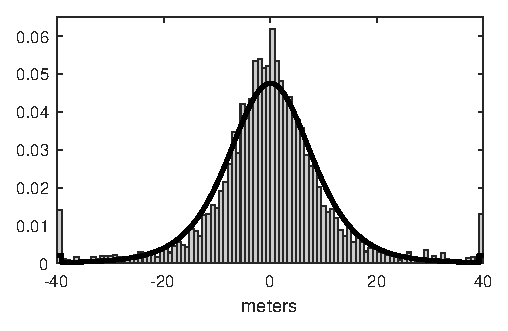
\includegraphics[width=19pc,angle=0]{tfit_error}}
  \centerline{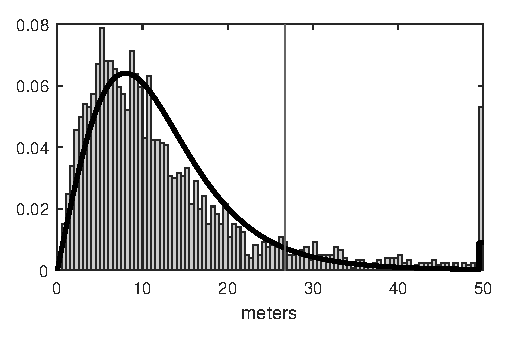
\includegraphics[width=19pc,angle=0]{tfit_distance_error}} 
  \caption{The top panel shows the position error distribution of the motionless GPS. The black line is the best fit t-distribution and the gray line is the best fit Gaussian distribution. The bottom panel shows the distance error distribution with the corresponding expected distributions from the Gaussian and t-distribution. The vertical line in the bottom panel shows the 95\% error of the t-distribution at about 29 meters.}
  \label{tfit_error}
\end{figure}

%%%%%%%%%%%%%%%%%%%%%%
\section{Tension Parameter}
%%%%%%%%%%%%%%%%%%%%%%

If we adjust the final tension parameter to so that the resulting error distribution matches the error distribution of the motionless GPS, this will result in an overly smoothed signal. We argue that the tension should vary based on the relative size of the measurement errors to the speed of motion. For example, if the position errors are only $1$ meter, but particle typically travels $10$ meters between measurements, then it is hardly justifiable to increase the tension so that the smoothing spline misses the observation points by $1$ meter. There is not enough statistical evidence to suggest that the true particle didn't go right through the observation point. On the other hand, if the position errors are  $1$ meter, but particle typically travels $10$ centimeters between measurements, nearby measurements are providing more information about the particle's true position during that time, so our estimate of the particles true position is closer to a mean of the nearby observations.

This idea can be made more rigorous by noting that there is a qualitative shift from smoothing to interpolating when the change in position, $\Delta x$, exceeds the position errors, $\sigma_x$. Assuming the physical process has a characteristic velocity scale, $u_{\textrm{rms}}$, we use this concept to define an interpolation condition $\Gamma$ as
\begin{equation}
\Gamma_x \equiv \frac{\sigma_x}{u_{\textrm{rms}}\Delta t}
\end{equation}
where $\sigma_x$ is the standard deviation of positioning noise, $u_{\textrm{rms}}$ is the typical particle velocity and $\Delta t$ is the typical time between observations. If $\Gamma<1$ then we are in the interpolation regime where the particle moves farther than the measurement noise between observations, and if $\Gamma >1$ we are in the smoothing regime where each observation is providing similar information to nearby observations. Loosely speaking, if $\Gamma=10$, then there are approximately 10 degrees of freedom that can be used to estimate the true position of the particle, assuming uncorrelated errors.

$\Gamma_x$ can be generalized to higher order derivatives so that,
\begin{equation}
\Gamma_{x^{(n-1)}} = \frac{  \sigma_{x^{(n-1)}} }{x^{(n)}_{\textrm{rms}} \Delta t }
\end{equation}
where $\sigma_{x^{(n-1)}}$ is the measurement noise of the of $(n-1)$-th derivative of the position error and $x^{(n)}_{\textrm{rms}}$ is the characteristic velocity, acceleration, jerk, etc. The interpretation is similar for each $n$. For example, at $n=2$, the interpolation condition occurs when changes in particle velocity exceed the velocity measurement noise.

This condition has a direct interpretation in terms of the total power of the physical process and the noise. Assume that the physical process has true value $x(t_i)$ at time $t_i$ and is stationary, but we observe value $x_i$ given by $x_i = x(t_i) + \epsilon_i$ where $\epsilon_i$ given by uncorrelated Gaussian noise with variance $\sigma_x$. Then the total power of the measured signal will be
\begin{equation}
 \frac{1}{N} \sum x_i^2 = \frac{1}{N} \sum \epsilon_i^2 + \frac{1}{N} \sum x(t_i)^2
\end{equation}
and similarly,
\begin{equation}
 \frac{1}{N} \sum u_i^2 = \frac{1}{N} \sum \left(\mathcal{D} \epsilon_i\right)^2 + \frac{1}{N} \sum u(t_i)^2
\end{equation}
where $u(t_i)$ and $u_i$ are the true and measured velocities of the process, respectively. This statement remains true for all higher order derivatives. Because the process is assumed to be stationary, the quantity describing the power of the process $\frac{1}{N} \sum u(t_i)^2$ is just $u_{\textrm{rms}}^2$. The power of the noise can be directly computed,
\begin{equation}
\frac{1}{N} \sum \left(\mathcal{D} \epsilon_i\right)^2 = \frac{2 \sigma_x^2}{(\Delta t)^2}
\end{equation}
where $\mathcal{D}$ is the first-order finite difference matrix and we've assumed sampling at even intervals $\Delta t$. This means that the square-root of the ratio of the total power of the noise to the total power of the signal is given by,
\begin{equation}
\tilde{\Gamma}_x \equiv \frac{\sqrt{2} \sigma_x}{u_{\textrm{rms}}\Delta t}.
\end{equation}
Once again this can be generalized to higher orders,
\begin{equation}
\tilde{\Gamma}_{x^{(n-1)}} = \frac{ \sqrt{\gamma_n} \sigma_x}{x^{(n)}_{\textrm{rms}} (\Delta t)^n }
\end{equation}
where $\gamma_n=\{2,6,20,70,252,..\}$ and is determined from the covariance structure of the finite differenced noise process.

The tension should be set so that the difference in power between the observed signal and the smoothed signal matches the expected power in the noise.

The tension parameter should be set based on the estimated size of the sample variance, using $\Gamma$ as the number of degrees of freedom,
\begin{equation}
\chi^2_{N-1} \sim (N-1) \frac{s^2}{\sigma_x^2}.
\end{equation}
(see `Distribution of Sample Variance' section in the wikipedia article on variance).

To what degree are nearby measurements helping me estimate the local value. This falls off in some nonlinear fashion, because we expect a Gaussian distribution.

Let's finish off by writing the following:
1. You can estimate urms by by looking at the spectrum and summing the components above the noise.
2. You get 1 DOF for estimating the mean and 2-3*$\Gamma$ additional DOF for estimating the variance of the noise. Going to $3 \sigma$ gives you a larger $\chi^2$ value, and is equivalent to increased smoothing---it's more conservative.
3. We tested this by considering the matern, so we show some figures and give the results.

\bibliographystyle{ametsoc2014}
\bibliography{references}

%\begin{acknowledgment} 
%Start acknowledgments here.
%\end{acknowledgment}
%
%% Use appendix}[A], {appendix}[B], etc. etc. in place of appendix if you have multiple appendixes.
%\ifthenelse{\boolean{dc}}
%{}
%{\clearpage}
%\begin{appendix}
%\section*{\begin{center}Appendix Title Is Entered Here (Primary heading)\end{center}}
%\subsection{First appendix secondary heading}
%
%\subsection{Second appendix secondary heading}
%
%\subsubsection{First appendix tertiary heading}
%
%\subsubsection{Second appendix tertiary heading}
%
%\paragraph{First appendix quaternary heading}
%
%\paragraph{Second appendix quaternary heading}
%
%\end{appendix}
%
%% Create a bibliography directory and place your .bib file there.
%% -REMOVE ALL DIRECTORY PATHS TO REFERENCE FILES BEFORE SUBMITTING TO THE AMS FOR PEER REVIEW
%\ifthenelse{\boolean{dc}}
%{}
%{\clearpage}
%\bibliographystyle{ametsoc}
%\bibliography{references}
%
%%%%%%%%%%%%%%%%%%%%%%%%%%%%%%%%%%%%%%%%%%%%%%%%%%%%%%%%%%%%%%%%%%%%%%
%% FIGURES-REMOVE ALL DIRECTORY PATHS TO FIGURE FILES BEFORE SUBMITTING TO THE AMS FOR PEER REVIEW
%%%%%%%%%%%%%%%%%%%%%%%%%%%%%%%%%%%%%%%%%%%%%%%%%%%%%%%%%%%%%%%%%%%%%%
%\begin{figure}[t]
%  \noindent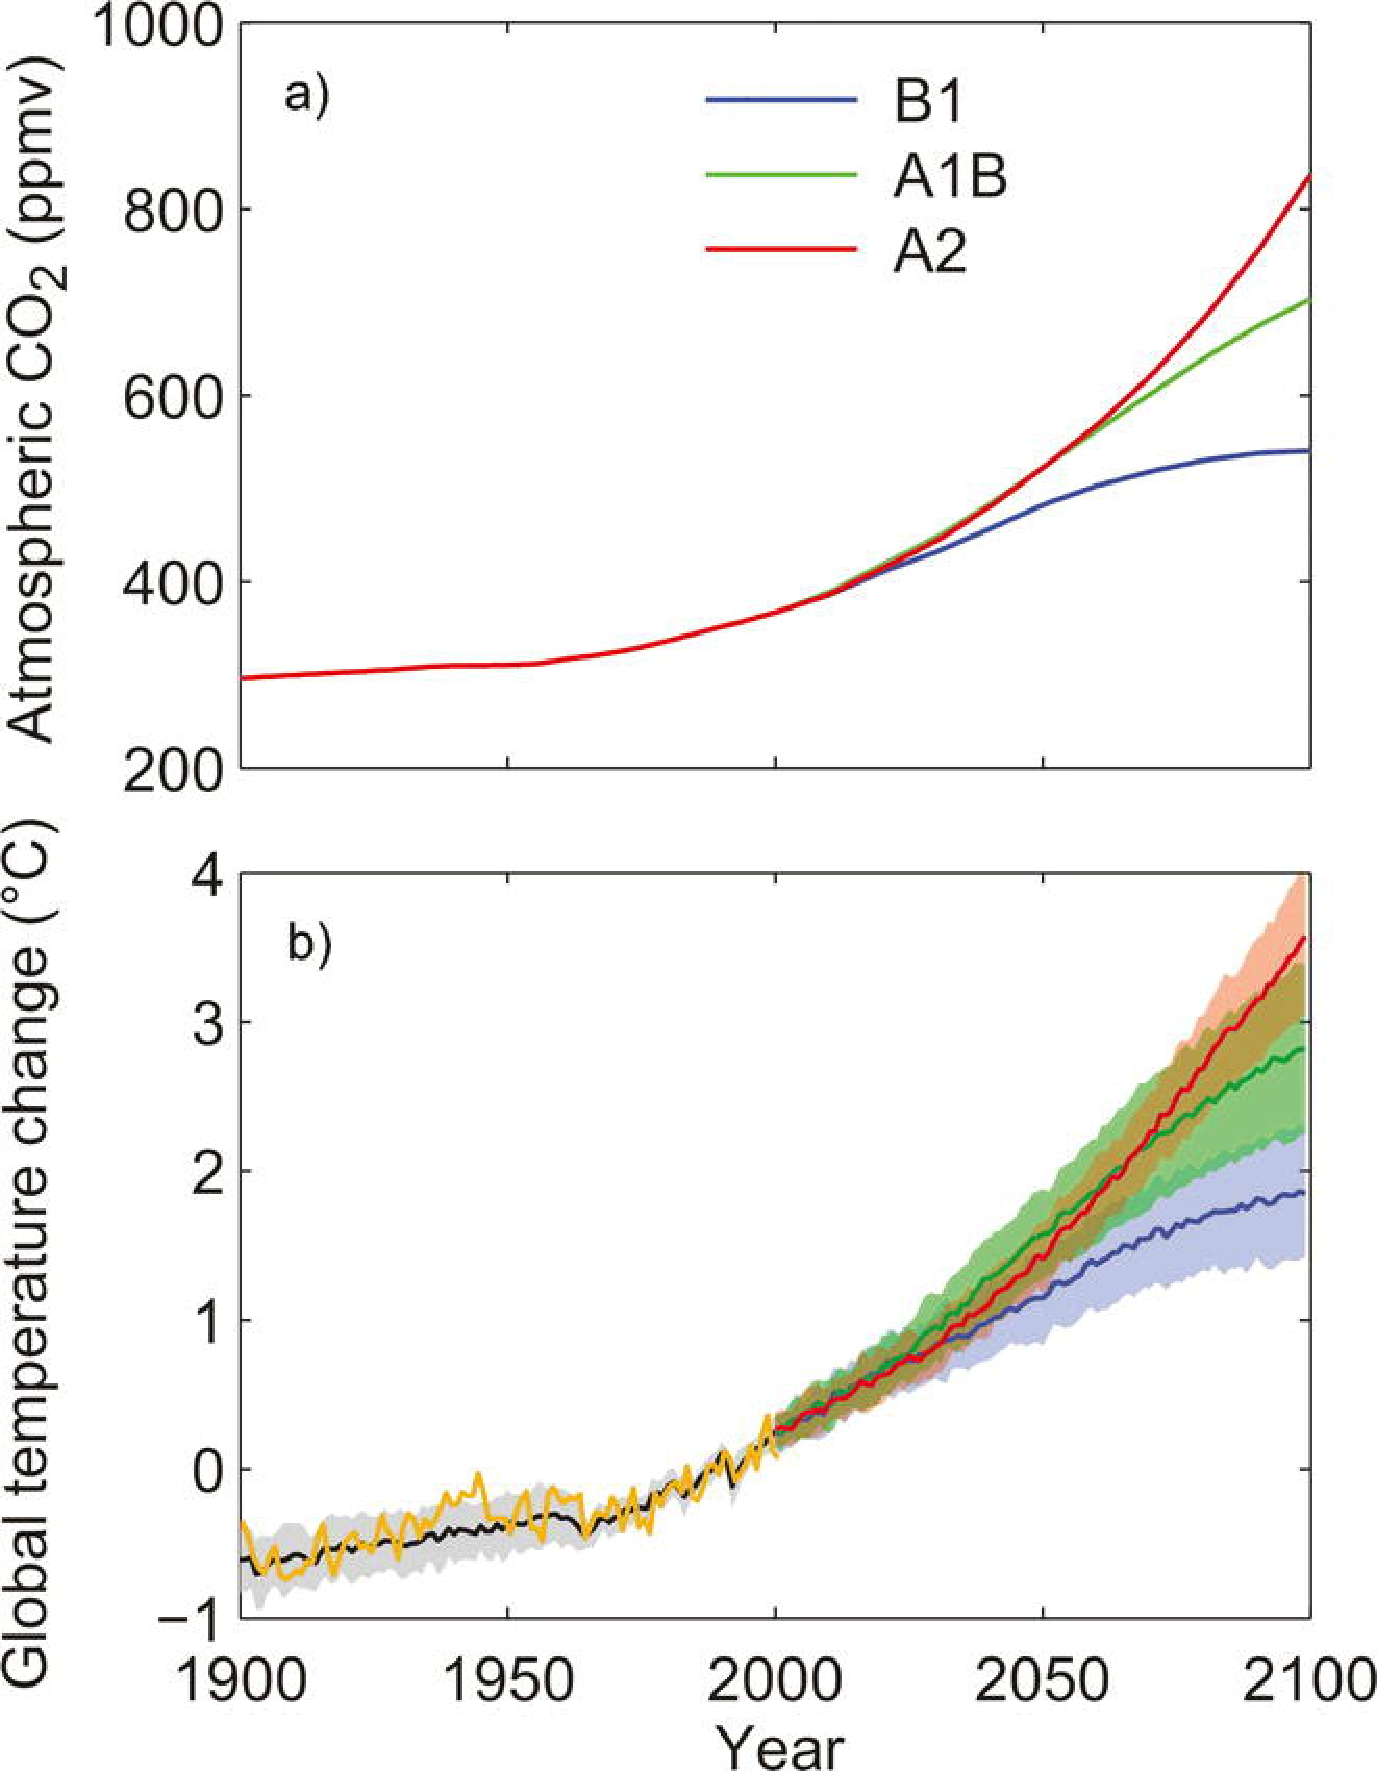
\includegraphics[width=19pc,angle=0]{figure01.pdf}\\
%  \caption{Enter the caption for your figure here.  Repeat as
%  necessary for each of your figures. Figure from \protect\cite{Knutti2008}.}\label{f1}
%\end{figure}
%%%%%%%%%%%%%%%%%%%%%%%%%%%%%%%%%%%%%%%%%%%%%%%%%%%%%%%%%%%%%%%%%%%%%%
%% TABLES
%%%%%%%%%%%%%%%%%%%%%%%%%%%%%%%%%%%%%%%%%%%%%%%%%%%%%%%%%%%%%%%%%%%%%%
%\begin{table}[t]
%\caption{This is a sample table caption and table layout.  Enter as many tables as
%  necessary at the end of your manuscript. Table from Lorenz (1963).}\label{t1}
%\begin{center}
%\begin{tabular}{ccccrrcrc}
%\hline\hline
%$N$ & $X$ & $Y$ & $Z$\\
%\hline
% 0000 & 0000 & 0010 & 0000 \\
% 0005 & 0004 & 0012 & 0000 \\
% 0010 & 0009 & 0020 & 0000 \\
% 0015 & 0016 & 0036 & 0002 \\
% 0020 & 0030 & 0066 & 0007 \\
% 0025 & 0054 & 0115 & 0024 \\
%\hline
%\end{tabular}
%\end{center}
%\end{table}
%
\end{document}